\section{Introduction}

\subsection{Abstract}
    Nowadays a need to analyze more complex data arises.
    Some objects and relations can not be represented as vectors in Euclidean space, and, therefore, we have to consider graps --- sets of nodes and connections between them --- as a subject of analysis.
    This poses a huge problem: we have to invent new algorithms, adapt known techniques and constantly improve them in order to work with such a complex data.

\subsection{Relevance}
    The field of research (graph neural networks) might be considered relatively new, and, therefore, there is a huge number of possible improvements to be made to existing models and approaches.
    Our ultimate goal is to improve the accuracy of node and graph classification.

    One of the proposed changes is to modify a Laplacian in such a way that it does not break existing model and improves it.
    Our initial results have shown that our approach indeed works well on Karate club dataset, where we had to classify nodes:

    \begin{figure}[h]
        \centering
        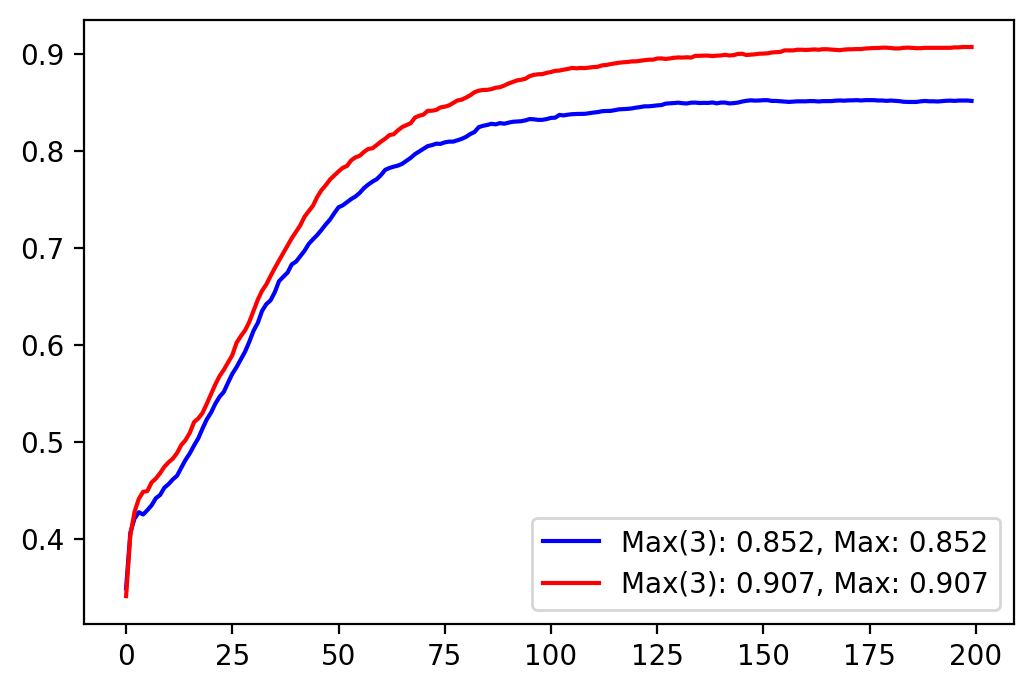
\includegraphics[width=0.6\textwidth]{custom_laplacian_accuracy.jpg}
        \caption{Default Laplacian (in blue) versus our Laplacian (in red). Y-axis is the accuracy, X-axis is the number of epochs}
    \end{figure}

\subsection{Subject of research}


